\documentclass[answers,12pt]{exam}

\usepackage{graphicx}
\usepackage{mhchem}

\pagestyle{headandfoot}
\runningheadrule
\firstpageheader{name:\fillin[][4cm]}{period:\fillin[][1cm]}{lesson 1.3: forces on matter}
\runningheader{lesson 1.3: forces on matter}
{Class Notes}
{Page \thepage\ of \numpages}
\firstpagefooter{}{}{}
\runningfooter{PACS}{Mr. Maxwell}{page \thepage\ of \numpages}


\begin{document}

\section{Lesson One}

\subsection{Composition of Matter}

\begin{questions}
  

  \question Matter is made of \fillin[atoms] that cannot be broken apart.
  \question Atoms are mostly \fillin[empty] space, but inside atoms 
  
  there are three kinds of particles:\\
       \fillin[protons] and \fillin[neutrons] are in the nucleus of the atom.
       \fillin[electrons] are outside the nucleus.

  


\end{questions}

\begin{center}
  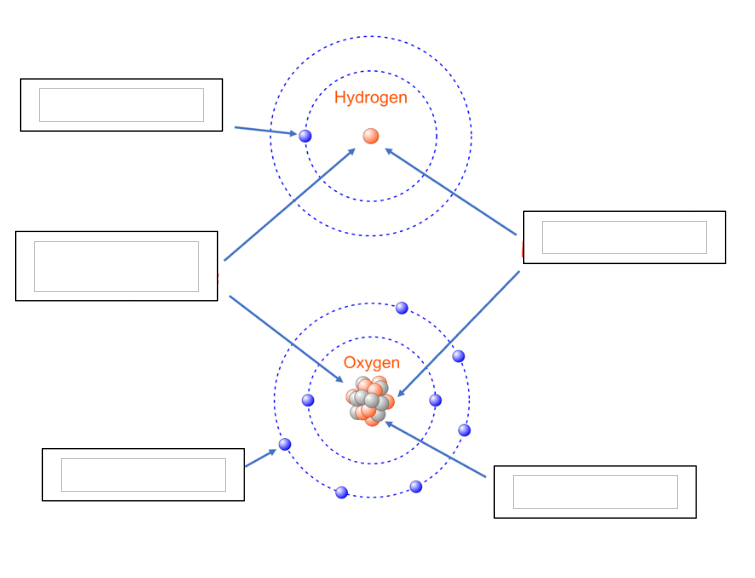
\includegraphics[width=1\textwidth]{atomLabel.png}
  
\end{center}

\begin{questions}
  

  \question The \fillin[mass] of an atom is almost all in the protons and neutrons in the nucleus.
  \question Electrons have a very \fillin[small] mass.
  \question The unit of mass is the \fillin[kilogram].
  \question Protons have a \fillin[positive(+)] electric charge and electrons have a \fillin[negative(-)] electric charge.

  \question Neutrons have a \fillin[neutral] charge
  \question Two or more atoms attached together are a \fillin[molecule].
  \question The connections between atoms in a molecule are called \fillin[chemical bond].
  \question Example a molecule of water ($H_2O$) has \fillin[two] hydrogen atoms and \fillin[one] oxygen atom.
  
\end{questions}

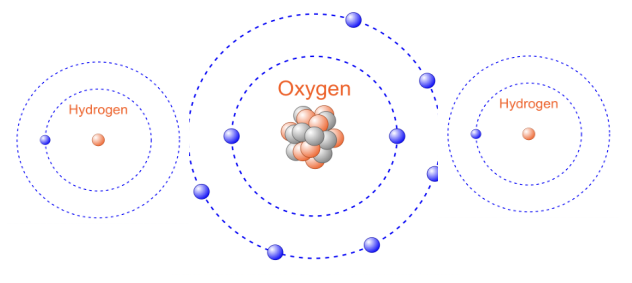
\includegraphics[width=1\textwidth]{water.png}

\begin{questions}
  

  \question The dimensions of matter are described as \fillin[length].
  \question The unit of length is the \fillin[meter] (m).
  \question The flat surfaces of matter are described as surface \fillin[area].
  \question The unit of surface area is \fillin[square meter] ($m^2$).
  \question The space matter occupies is described by its \fillin[volume].
  \question The unit of volume is \fillin[cubic meter] ($m^3$).

\end{questions}

\pagebreak

\subsection{Volume, Mass and Density}

\begin{questions}
  
  
  \question The \fillin[density] of a material is defined as:

  $density = \frac{mass}{volume}$
  
  \question If the density of a substance is \fillin[less] than the density of a liquid, the substance \fillin[float] on the liquid.
  
  \question If the density of a substance is \fillin[greater] than the density of a liquid, the substance \fillin[sink] in the liquid.


  \titledquestion{Cell Phone} Cell Phone 

  $$ V = volume = 150 \; cm^3 $$
  $$ M = mass = 200 \;g $$
  $$Density_{phone} = \fillin[1.33 g/ml] $$ 

  \question will the phone sink? \fillin[yes]

  \titledquestion{Pencil} Pencil 

  $$ V = volume = 10 \; cm^3 $$
  $$ M = mass = 7 \;g $$
  $$Density_{phone} = \fillin[0.7 g/ml] $$

  \question will the pencil sink? \fillin[no]
  
\end{questions}


\pagebreak

\begin{questions}


    \section*{Warm Up}

    \question What are the three particle that make up an atom? Which one is positive, negative, and neutral?

   \begin{center}
    \begin{tabular}{|c|c|}
        \hline
        particle & charge \\ \hline
        \hspace{2cm} & \hspace{2cm} \\ \hline
        \ & \ \\ \hline
        \ & \ \\ \hline

    \end{tabular}
   \end{center}


    \question Draw a picture of a \ce{^4_2He} atom. Label the nucleus, protons, neutrons and electrons.

    \vspace{3cm}

    \subsection{Forces on Matter}

    \question A force is a \fillin or a \fillin on an object.

  \begin{center}
    
\includegraphics[width=0.5\textwidth]{pushpull}
  \end{center}


    \question We draw a force with an arrow that shows the \fillin of the force.
    
    
    \question There are two kinds of forces:
    \begin{parts}
        \part \fillin[][4cm] force
        \part \fillin[][4cm] force
    \end{parts}
    

\subsection*{Gravitational Force}

\question Gravity is a force on the \fillin of an object caused by the mass of \fillin object.
\question Gravity is always a \fillin force between two masses.
\question The gravitational force between two masses happens no matter how \fillin the masses are from each other.
\question The gravitational force gets \fillin when the masses get farther apart.
\question On Earth the gravitational force on objects is always \fillin.

\subsection*{Electromagnetic Force}

\question The electromagnetic force is caused by the pushing and pulling between the electric charges of \fillin and \fillin in an object no matter how far apart they are.
\question The electromagnetic force gets \fillin when the electric charges are farther apart.
\question Two positive charges (protons) will \fillin (repel) each other away.
\question Two negative charges (electrons) will \fillin (repel) each other away.
\question A positive charge (proton) and a negative charge (electron) will pull (\fillin) each other.

\subsection*{Examples of Electromagnetic Force}

\question \fillin electric charges (protons) in a metal can pull on (\fillin) negative electric charges (electrons) in a balloon.
\question The positive (protons) and negative (\fillin) electric charges in a magnet can either push the magnets apart (\fillin) or pull them together (attract).
\question The negative electric charges (electrons) in your hand \fillin on the negative electric charges (electrons) in an object that you touch.
\question When you stretch a rubber band the protons attract the electrons and \fillin back.

\pagebreak

\subsection{Temperature and Matter}


\question Temperature measures the \fillin of the \fillin of atoms and \fillin in a material.

\question The modern metric system unit of temperature is degrees \fillin (°C) or degrees \fillin (°K).

\question Degrees Kelvin (°K) = degrees Celcius (°C) + \fillin°

\question The symbol for temperature is \fillin.


\end{questions}

\subsection*{Phet Temperature Simulation}

\begin{enumerate}
  \item Click on the “States” box.
  \item Click on “Water” in in the box in the upper right.
  \item Use the “Heat” or “Cool” controls to add or remove energy from the water. Observe what happens to the water temperature and to the water molecules. Try using the “Cool” control to lower the temperature to 0 K.
  \item Note that you can change the units of the temperature to either Celsius or Kelvin.
\end{enumerate}

\subsection*{Answer the questions below}

\begin{questions}
  \question What happens to the molecules of matter when the temperature goes up?

  \vspace{3cm}

  \question What happens to the molecules of matter when the temperature goes down?
\end{questions}

\pagebreak

\subsection{States of Matter}

\begin{questions}
  
  \question Matter has three states: \fillin, \fillin, and \fillin (vapor).  We want to understand what determines which state matter is in.

  \question In a material there are electromagnetic forces between molecules.  These forces are called \fillin forces.
  
  \question In solids the intermolecular forces are \fillin, so solids cannot change their shape or volume.
  
  \question In liquids the intermolecular forces are moderately strong, so liquids can change their shape but not their \fillin.
  
  \question In gasses the intermolecular forces are \fillin, so gasses can change their shape and volume.
  
  \question When the temperature of matter increases, the molecules move \fillin and the intermolecular forces become weaker.
  
  \question When the temperature of a solid increases the solid becomes a liquid by \fillin.  
  
  \question When the temperature of a liquid increases the liquid becomes a gas by \fillin or by evaporation.
  
  \question When the temperature of a gas decreases the gas becomes a liquid by \fillin.
  
  \question When the temperature of a liquid decreases the liquid becomes a solid by \fillin.
  
  \question Solids can become gas without first becoming liquid.  This is called \fillin.  Dry ice is an example of sublimation.
  
  \question A physical change in matter is when there is a change in the form of the matter but no chemical bonds are broken, so the molecules of the material stay the \fillin.
  
  \question Melting, evaporation, boiling, condensation, and freezing are examples of \fillin changes.
  
  \question Other examples of physical changes are:
      ◦ Adding food \fillin to cake batter
      ◦ \fillin a material into smaller pieces like slicing bread
      ◦ \fillin materials like in preparing cake batter
      ◦ \fillin an egg

  \question What example of a physical change can you think of?  Write your answer below.



\end{questions}

\end{document}